%%%%%%%%%%%%%%%%%%%%%%%%%%%%%%%%%%
\subsection{APA Frame Mounting Structure and Module Securing}	
\label{sec:fdsp-pd-assy-frames}
%\todo{\color{blue} Content:  Warner}

\Dword{pd} modules are inserted into the \dword{apa} frames through ten slots (five on each side) and are supported inside the frame by stainless steel guide channels.  The slot dimensions for the \dword{spmod} \dword{apa} frames 
are \SI{136.0}{mm}$\times$\SI{25.0}{mm}\footnote{For \dword{pdsp} they were only \SI{108.0}{mm}$\times$\SI{19.2}{mm} wide; the increase allows for larger \dword{pd} modules and an increase in light collection area of nearly 50\% over the \dword{pdsp} design.}   
(see Figure~\ref{fig:pds-pd-mounting}(left)).
The guide channels are positioned into the \dword{apa} frame prior to application of the wire %shielding 
mesh, % to the \dword{apa} frames, 
and are not accessible following wire wrapping. Following insertion, the \dword{pd} modules are fixed in place using two stainless steel captive screws.

%, as shown in Figure~\ref{fig:pds-pd-mounting}(right).
 
 %\fixme{\color{blue}Dave W:  Will replace prior to second draft1/15/19 with similar but corrected images for current X-ARAPUCA design}

\begin{dunefigure}[\dword{pd} mounting rails in \dword{apa} frame.]{fig:pds-pd-mounting}
{\dword{pd} mounting in \dword{apa} frame: Fixed end of PD module inside transparent APA side tube showing clearance for C\dword{ce} cables (left) and showing \dword{pd} mounting rails in an APA frame  (right).}
	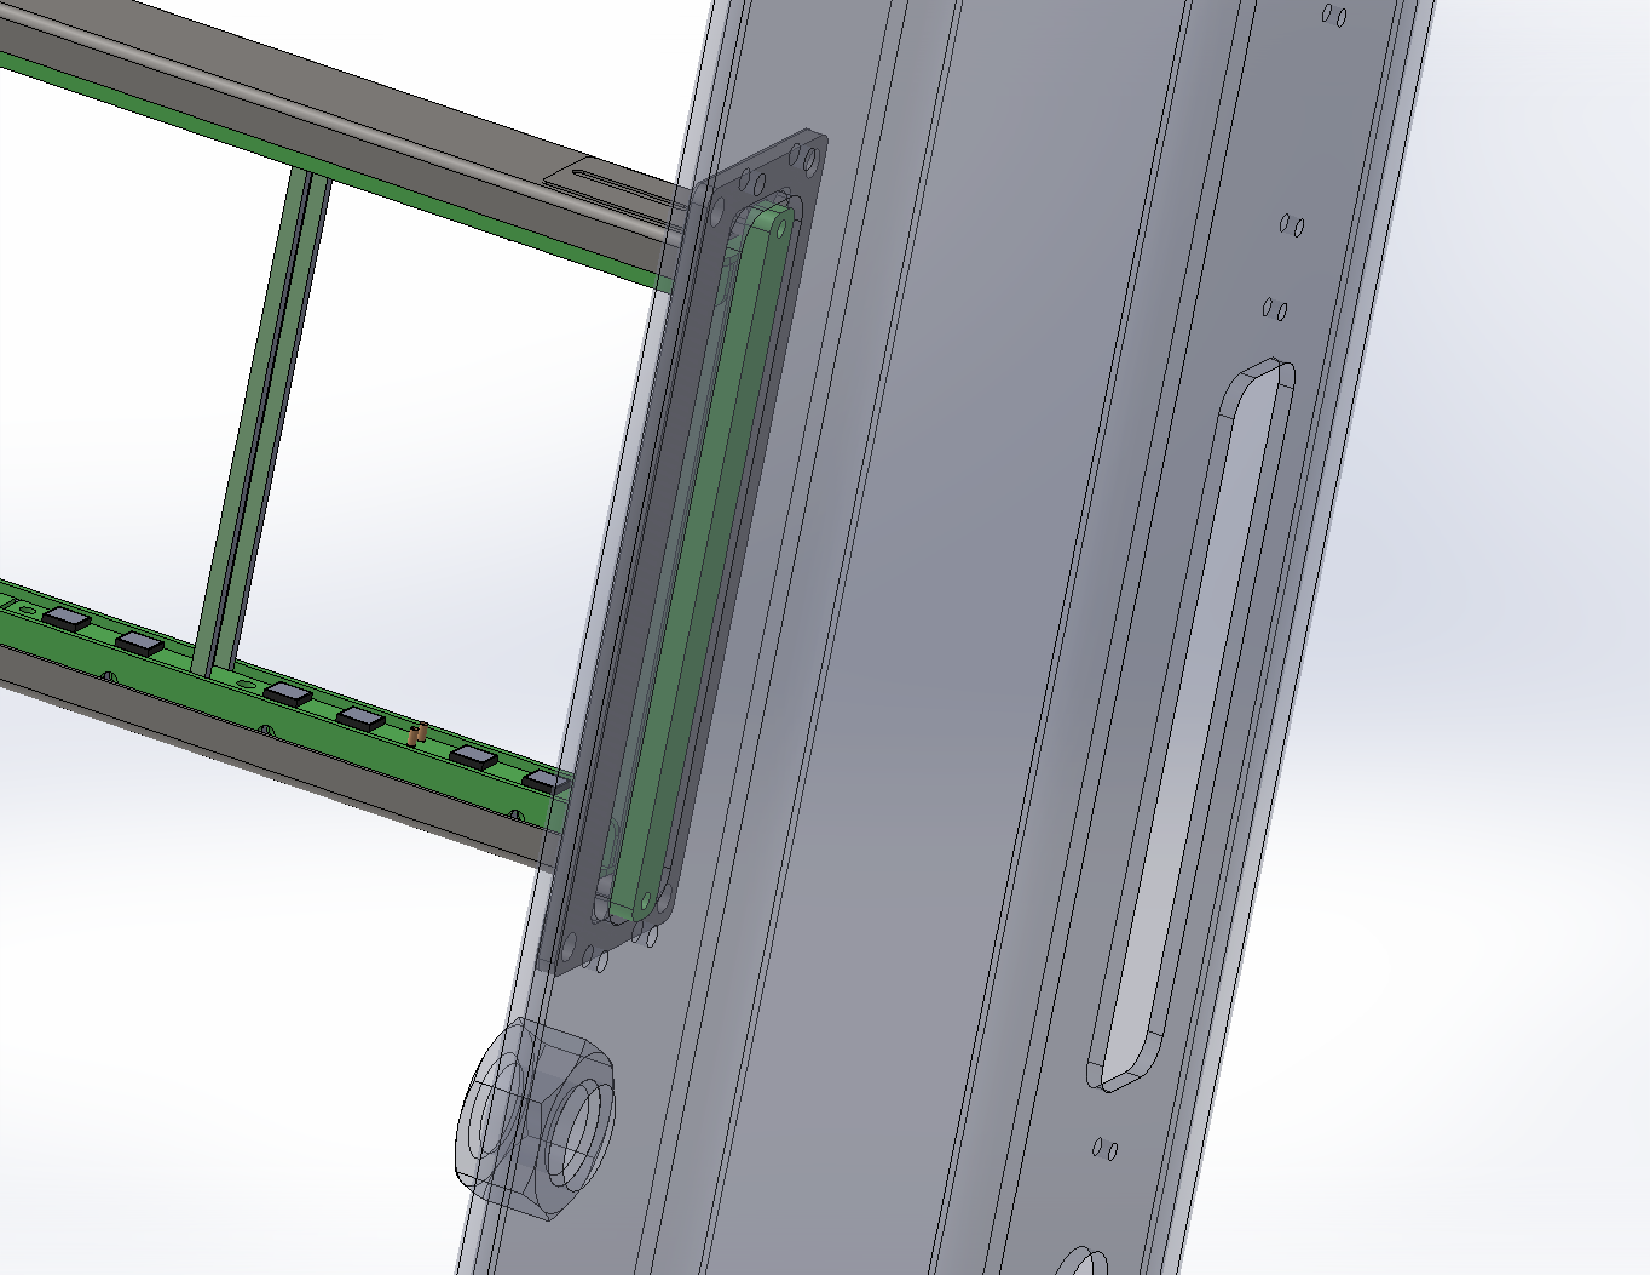
\includegraphics[height=6.5cm]{pds-apa-pd-mounting-fixation}
	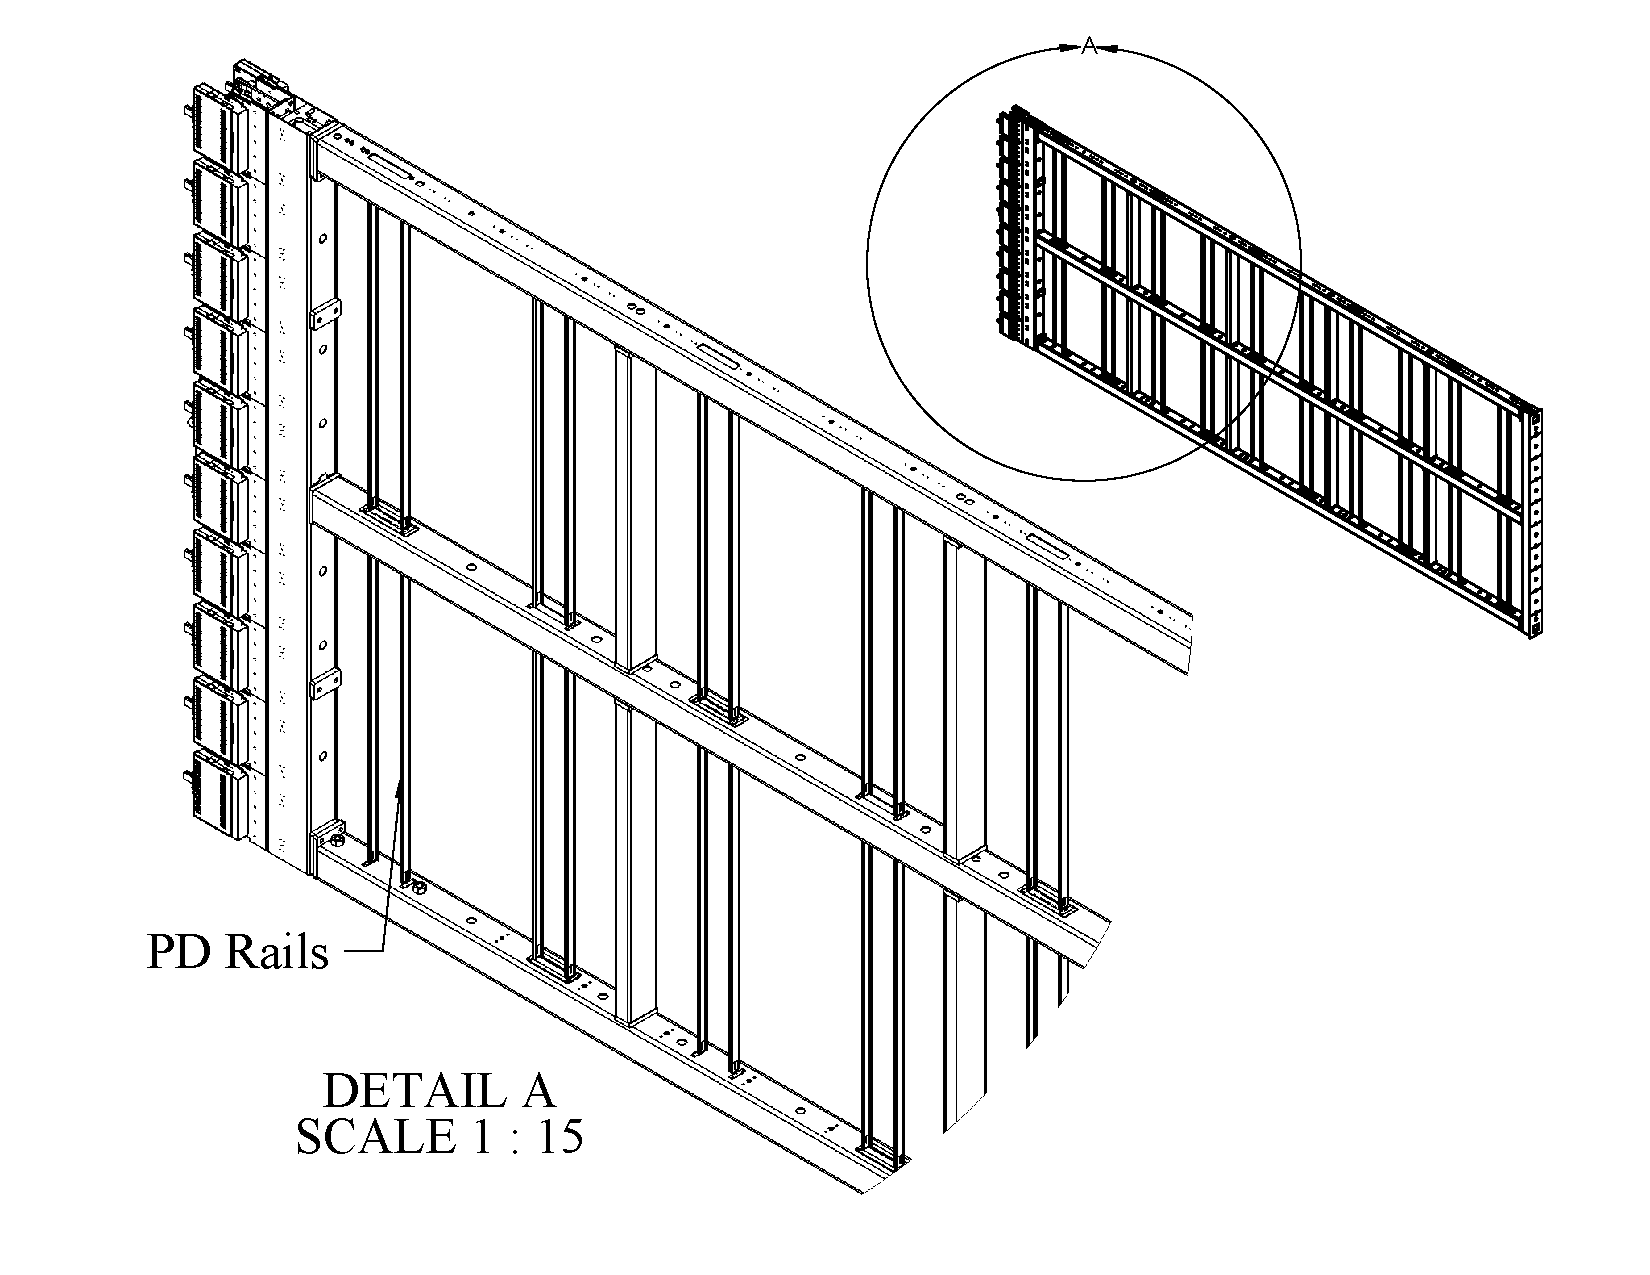
\includegraphics[height=6.5cm]{pds-apa-pd-rails}
\end{dunefigure}

\subsubsection{Signal cable and connections}

For the \dword{pdsp} ,\dword{pd} cables were run inside the \dword{apa} side tubes, five cables per side.  For the \dword{spmod}, however, this space will be filled by \dword{ce} cables.  This change required a revised plan for locating the \dword{pd} cables.  In addition, it was observed during \dword{pdsp} \dword{pds} installation that running the \dword{pd} cables and making electrical connections to the modules during \dword{pd} integration was time-consuming and introduced risk to the process.

For the \dword{spmod}, the \dword{pd} cables will be %pre-
positioned in the \dword{apa} frames prior to installing the %ground shield 
mesh and wire-wrapping the frame.  %This will require two different styles of \dword{apa} frame: (1) those intended to be installed in the bottom position in an \dword{apa} stack which will house the cables for only the lower \dword{apa} and those intended to be installed in the top position, which will house the cables for both the upper \dword{apa} \dword{pd}s and the pass-through cables from the lower \dword{apa}, all cables terminating at the header of the top \dword{apa} after assembly (see Figure~\ref{fig:pd-cable-routing-apa-frames}).
An \dword{apa} in the lower position will house the cables for only the \dwords{pd} in that lower \dword{apa} whereas those in the top position will house the cables for the upper \dword{apa} \dword{pd}s and the pass-through cables from the lower \dword{apa}. The cabling thus requires two different styles of \dword{apa} frame. All cables terminate at the header of the top \dword{apa} after assembly (see Figure~\ref{fig:pd-cable-routing-apa-frames}).

The cable connections between the upper and lower \dword{apa}s are made during \dword{apa} installation into the cryostat, while the \dword{apa} stack is being assembled. The same in-line multi-pin connectors used at the flange penetration in \dword{pdsp}\footnote{Hirose LF 10WBP-12S connectors https://www.hirose.com} are used for this connection.
%\{Dave: Do you want to put more specific info in the footnote on the connector?}

The \dword{pd} signal cables are expected to thermally contract approximately 2\% during cool-down of the \dword{detmodule} to cryogenic temperatures.  The design accounts for this by leaving cable loops in place between the anchor points to the \dword{apa} frame, allowing for the required relative motion.

%\fixme{need to put in figures of cables in \dword{apa} frames here}

\begin{dunefigure}[\dword{pd} cable routing in \dword{apa} frames.]
{fig:pd-cable-routing-apa-frames}
{\dword{pd} cable routing in \dword{apa} frames: Bottom \dword{apa} (left) and top \dword{apa} (right).}
	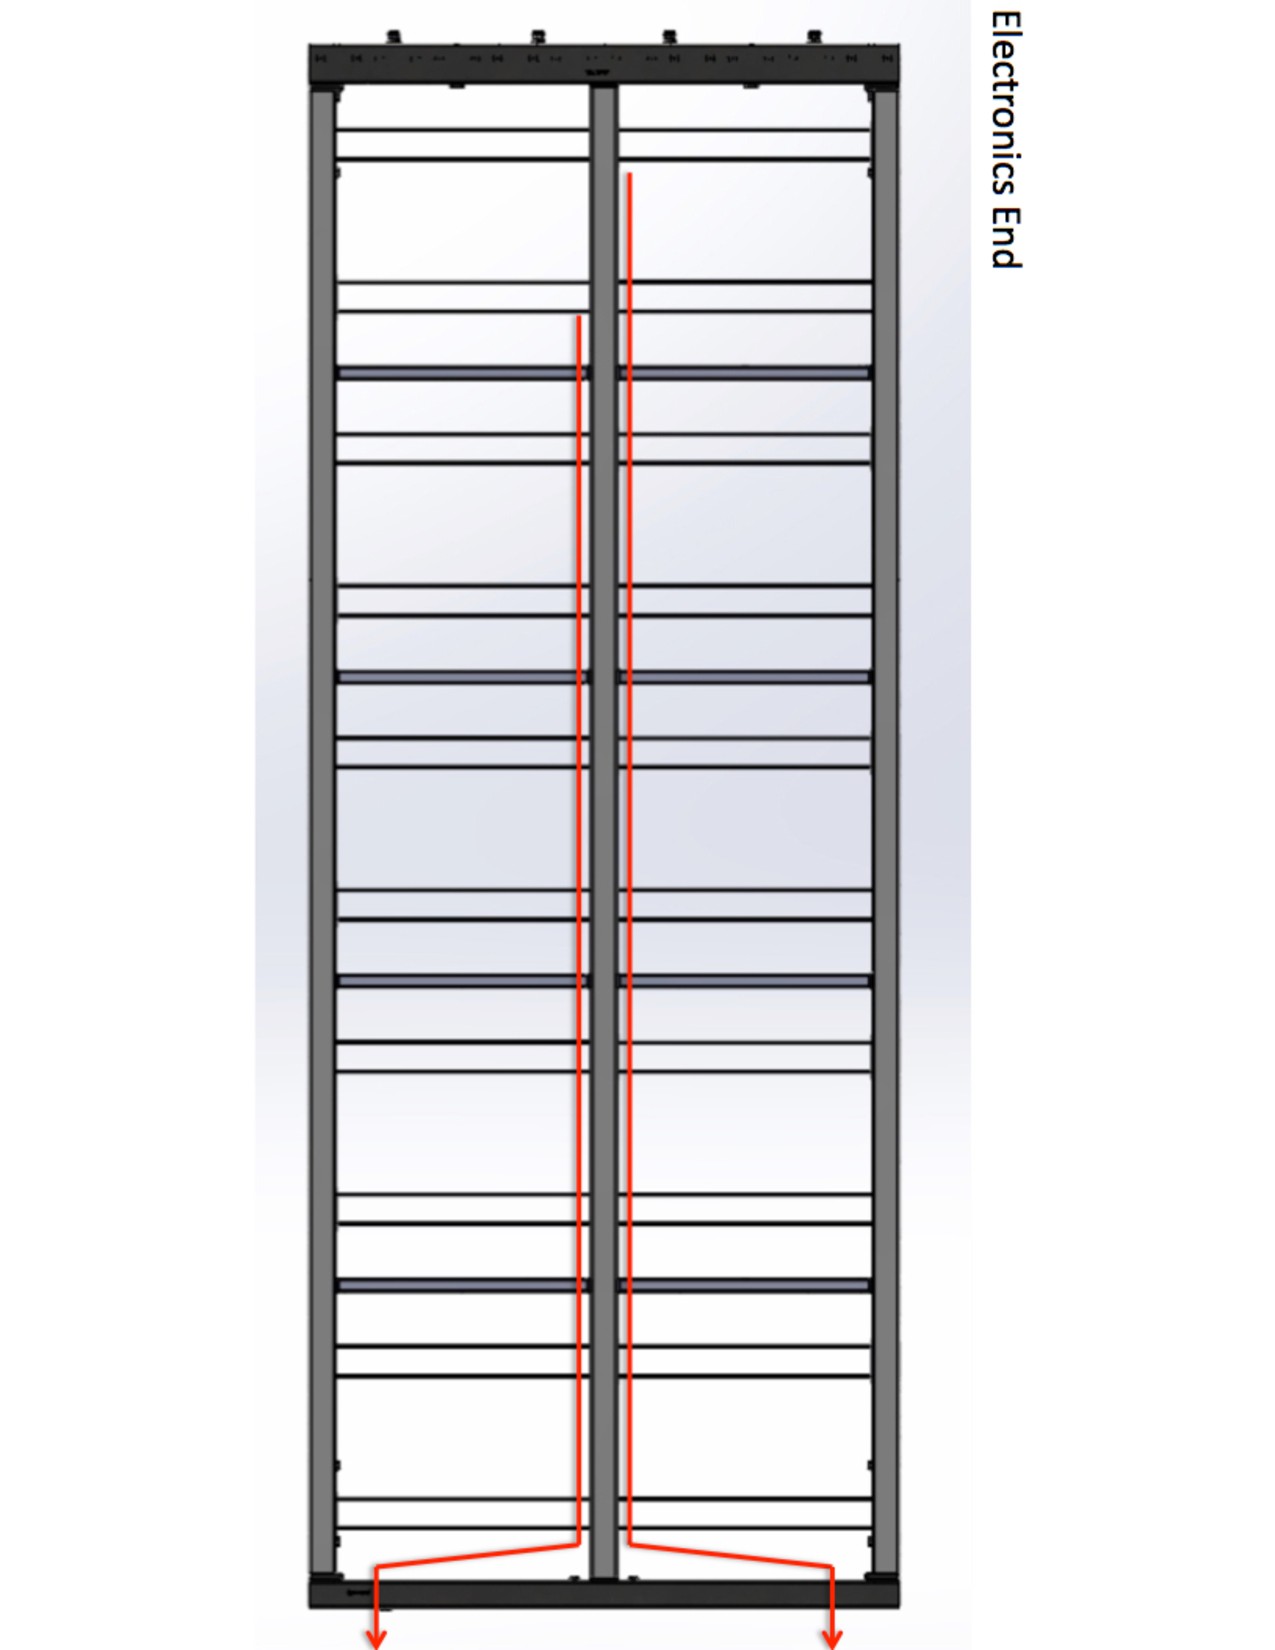
\includegraphics[angle=90,height=6.6cm]{pds-lower-apa-pds-cable-routing}
	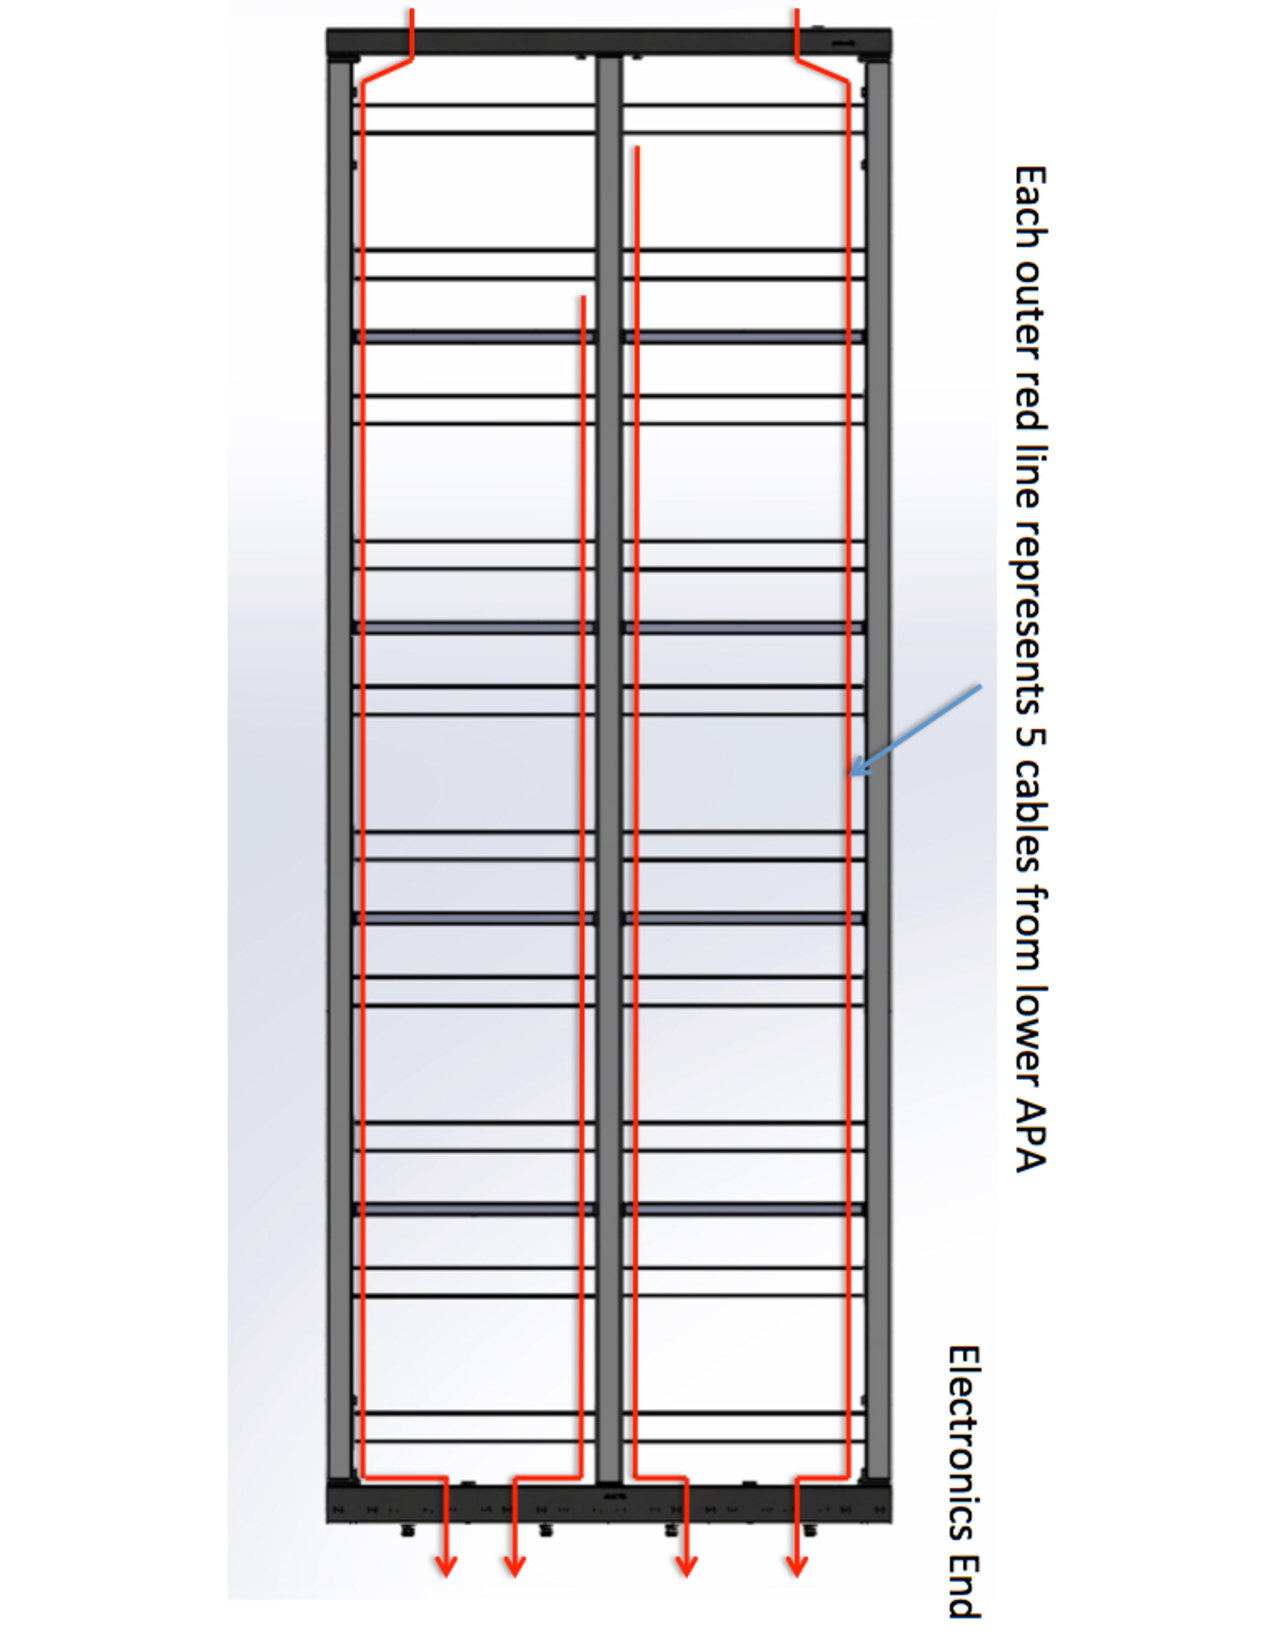
\includegraphics[angle=90,height=6.6cm]{pds-upper-apa-pds-cable-routing}
	\vspace{-1.5cm}
\end{dunefigure}

To remove interference with the \dword{ce} cables, the electrical connections between the \dword{pd} modules and the pre-positioned cable harness are moved to the face of the central \dword{apa} tube.  Printed circuit boards with spring-loaded electrical sockets are pre-positioned on the inside face of the tube as part of the \dword{pd} rail installation as shown in Figure~\ref{fig:pd-cable-connectors.} (left).  During \dword{pd} integration into the \dword{apa} frames, a PCB with pin contacts mounted to the \dword{pd} module (see figure~\ref{fig:mounting-board-routing-board} right) engages into the PCB mounted to the \dword{apa} frame, automatically making the electrical connection as shown in 
Figure~\ref{fig:pd-cable-connectors} (right).

%\{Dave: you have three figure references in the paragraph - I am not certain which goes with which so I will leave that for you.}

\begin{dunefigure}[\dword{pd} cable connectors.]{fig:pd-cable-connectors}
{\dword{pd} cable connectors in \dword{apa} frames: \dword{pd} connector plate mounted in \dword{apa} frame (ICEBERG model, left) and installed \dword{pd}/connector assembly in \dword{apa} (right).  Note that active ganging PCBs are buried inside the central tube.}
	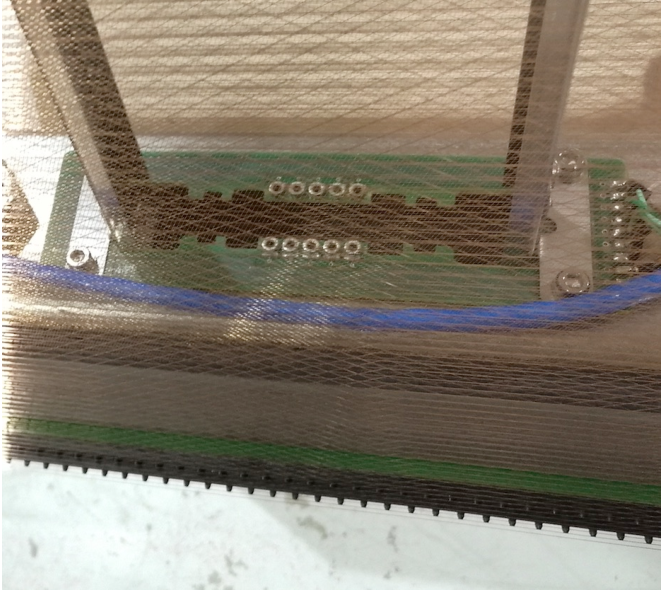
\includegraphics[height=7.5cm]{pds-connector-mounted-in-apa.pdf}
	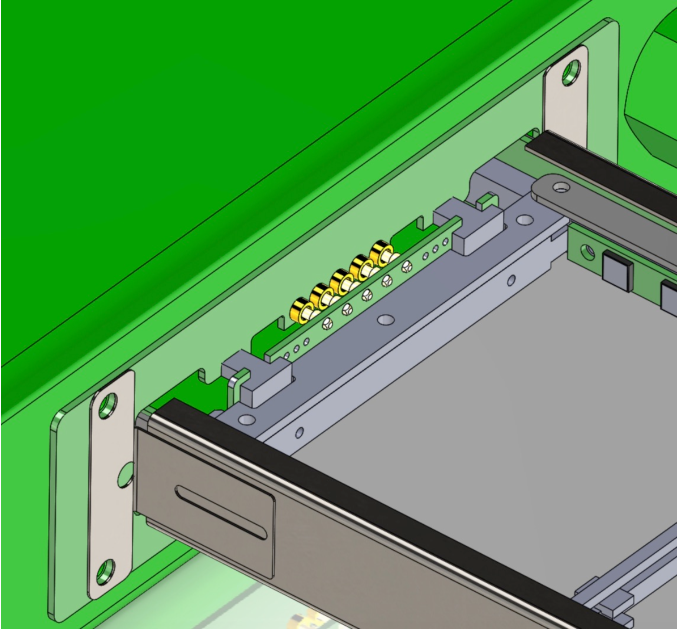
\includegraphics[height=7.5cm]{pds-connector-assembly-in-apa.pdf}
\end{dunefigure}

\subsubsection{Thermal Contraction and Load Deformation}

\textit{\bf Thermal Contraction}

During cooldown from room 
%temperature 
to \dword{lar} temperatures,  significant relative shrinkage of module components is possible.  Mitigating these effects was a major consideration in the \dword{xarapu} module design.

Thermal expansion coefficients (CTEs) for the stainless steel \dword{apa} frames and fused-silica filter plates drove the materials selection for the \dword{xarapu} modules.  The frame components are fabricated from FR-4 G-10, resulting in a shrinkage of the stainless steel frame structure relative to the frame of approximately \SI{1.2}{mm} along the long ($\sim$\SI{2}{m}) axis of the bar.  The shrinkage of the frame relative to the filter plate is <\SI{0.2}{mm}.  Both these relative shrinkage factors are accounted for in the dimensions and tolerances of the design.

The largest relative contraction of mechanical components is between the FR-4 frame and the acrylic \dword{wls} plates. However, the most critical relative shrinkage is between the face of the photosensors and the \dword{wls} plate, where the significantly greater contraction of the \SI{92}{mm} width of the plate relative to the \dword{pd} module structure will result in an increase in separation between the sensor face and the plate of approximately \SI{1.3}{mm}.  
 Simulation and testing are ongoing to understand the impact this will have on the performance of the \dword{xarapu}.  Relative contraction along the long axis of the \dword{wls} plate (\SI{487.0}{mm} long plate, resulting in a \SI{5.8}{mm} relative contraction) is addressed by the \dword{wls} bar mounting structure.

\begin{dunetable}[Shrinkage of \dword{pd} materials]
%{|c|c|}
{lc}
{tbl:fdsfpdshrink}
{Shrinkage of \dword{pd} module materials for a $206^{\circ}$C temperature drop}
Material 			 & Shrinkage Factor (m/m)\\ \toprowrule
Stainless Steel (304) & $2.7\times10^{-3}$\\ \colhline
FR-4 G-10 (In-plane) & $2.1\times10^{-3}$\\ \colhline
Fused Silica (Filter Plates) & $1.1\times10^{-4}$\\ \colhline
Acrylic (WLS Bars) & $1.4\times10^{-2}$\\ \colhline
\end{dunetable}

  Mitigation of these contractions is detailed in Table~\ref{tbl:fdsfpdshrinkeffects}.

\begin{dunetable}[Relative shrinkage of \dword{pd} components and \dword{apa} frame]
%{|p{0.2\textwidth}|p{0.2\textwidth}|p{0.5\textwidth}l}
{p{0.2\textwidth}p{0.2\textwidth}p{0.5\textwidth}}
{tbl:fdsfpdshrinkeffects}
{Relative Shrinkage of \dword{pd} components and \dword{apa} frame, and mitigations.}
\textbf{Interface} & \textbf{Relative shrinkage} & \textbf{Mitigation} \\ \toprowrule
\dword{pd} Length to \dword{apa} width & \dword{pd} expands  \SI{1.2}{mm} Relative to \dword{apa} frame & \dword{pd} affixed only at one end of \dword{apa} frame, free to expand at other end.  \SI{3}{mm} nominal clearance (beyond tolerance allowance) for expansion in design \\ \colhline
Width of \dword{pd} in \dword{apa} Guide Rails & \dword{pd} expands \SI{.1}{mm}  relative to slot width & \dword{pd} not constrained in C-channels. C channels and tolerances designed to contain module across thermal contraction range \\ \colhline
Width of module end mount board to stainless steel frame & Stainless frame shrinks \SI{0.1}{mm}  more than PCB & Diameter of shoulder screws and FR-4 board clearance holes selected to allow for motion \\ \colhline
Length of WLS bar relative to FR-4 \dword{pd} frame & WLS bar shrinks \SI{5.8}{mm} relative to \dword{pd} frame & Allowed for in WLS bar mount fixtures \\ 
\end{dunetable}

%\subsubsection{\dword{pd} Mount frame deformation under static \dword{pd} load}

\textit{\bf \dword{pd} Mount frame deformation under static \dword{pd} load}

%\fixme{Dave: Section will remain but requires new calculations based on X-ARAPUCA design.  Will be complete by March 2019 revision. -Dave} rhw This is on Dave's todo list.

\Dword{fea} modeling of the \dword{pd} support structure was conducted to study static deflection 
prior to building \dword{pdsp} prototypes.  Modeling was conducted in both the vertical
 orientation (\dword{apa} upright, as installed in cryostat) and also horizontal orientation.  
Basic assumptions used were fully-supported fixed end conditions for the rails, 
with uniform loading of 3X \dword{pd} mass (\SI{5}{kg}) along rails.  
Figure~\ref{fig:pds-rail} illustrates the rail deflection for the \dword{apa} in the horizontal (left) and vertical (right) orientations.
Prototype testing confirmed these calculations.  Similar modeling of final-design \dword{dune} pd modules will be completed prior to the final draft of the \dword{tdr}.

\begin{dunefigure}[\dword{pd} mechanical support analysis.]{fig:pds-rail}
{\dword{pd} mechanical support analysis: Rail deflection for the \dword{apa} in the horizontal (left) and vertical (right) orientations.}
	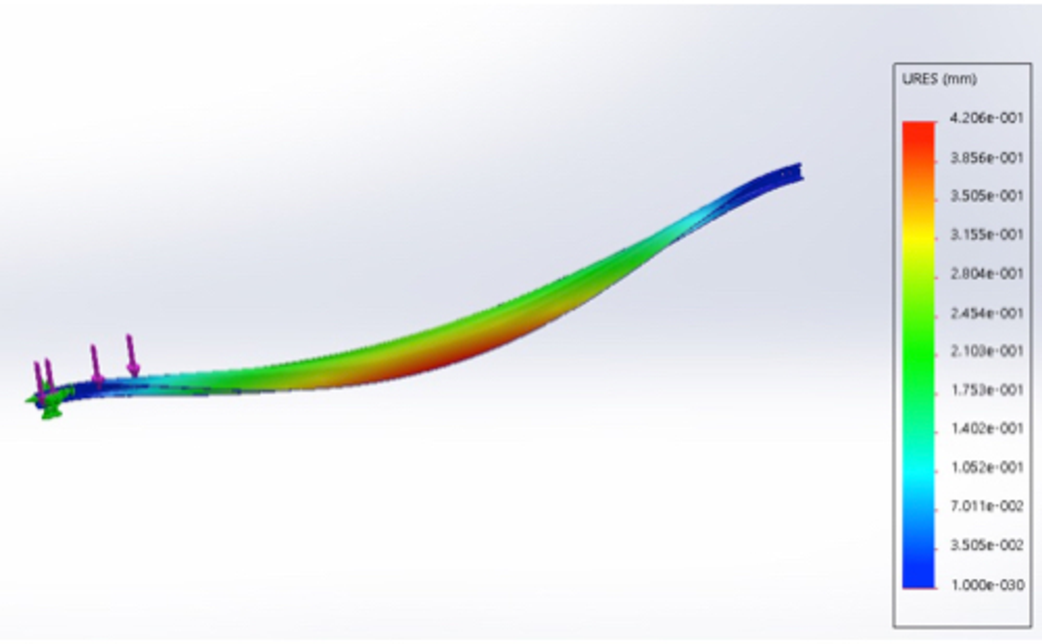
\includegraphics[height=4.5cm]{pds-rail-deflec-apa-flat.pdf} 
	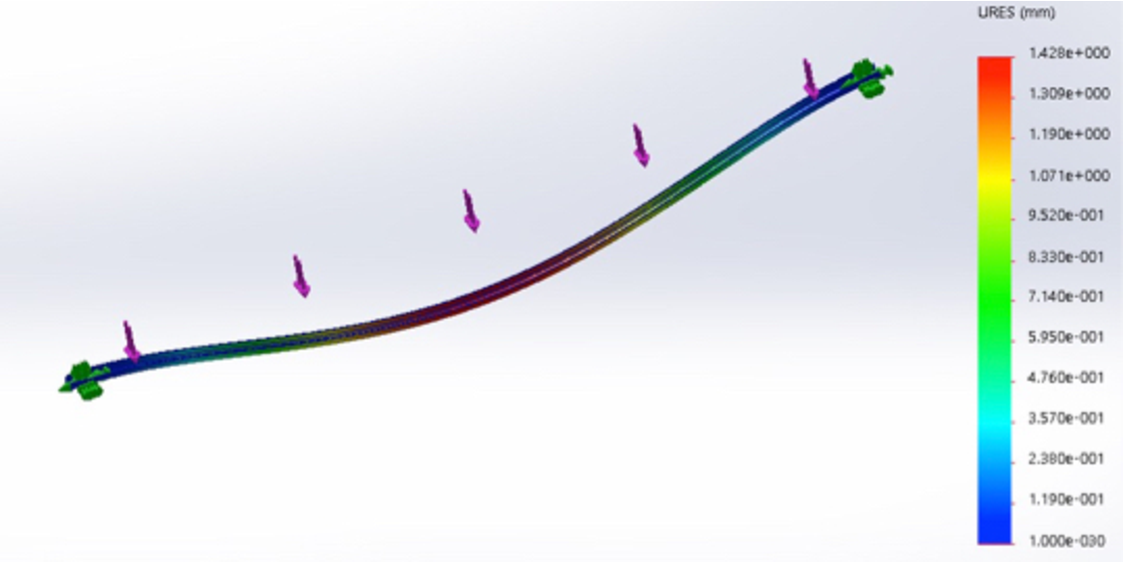
\includegraphics[height=4.5cm]{pds-rail-deflec-apa-vert.pdf}\\
%	%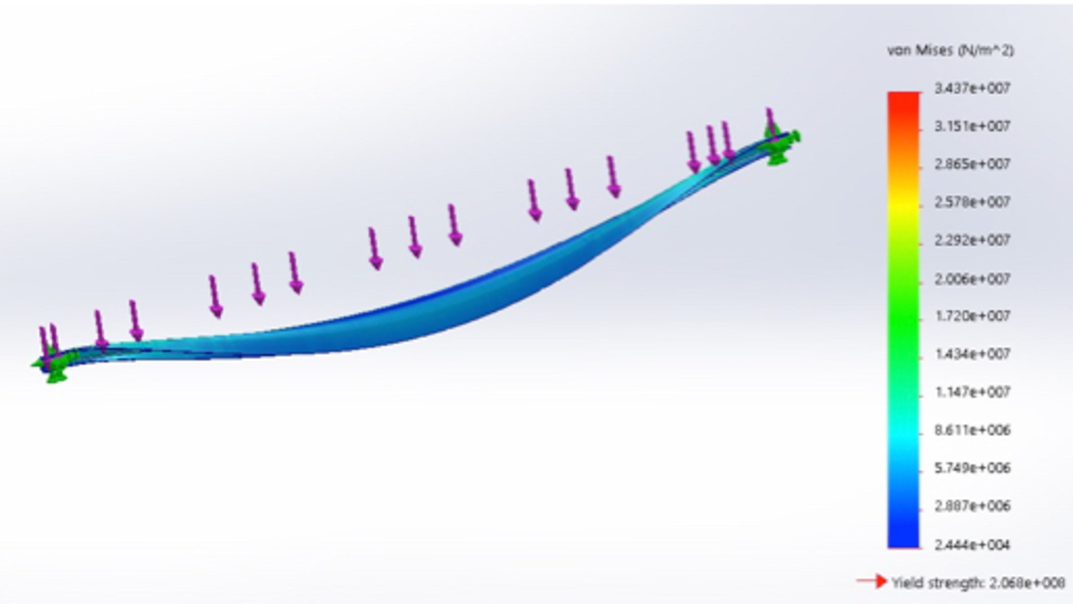
\includegraphics[width=0.25\columnwidth]{pds-rail-stress-apa-flat.pdf} 
%	%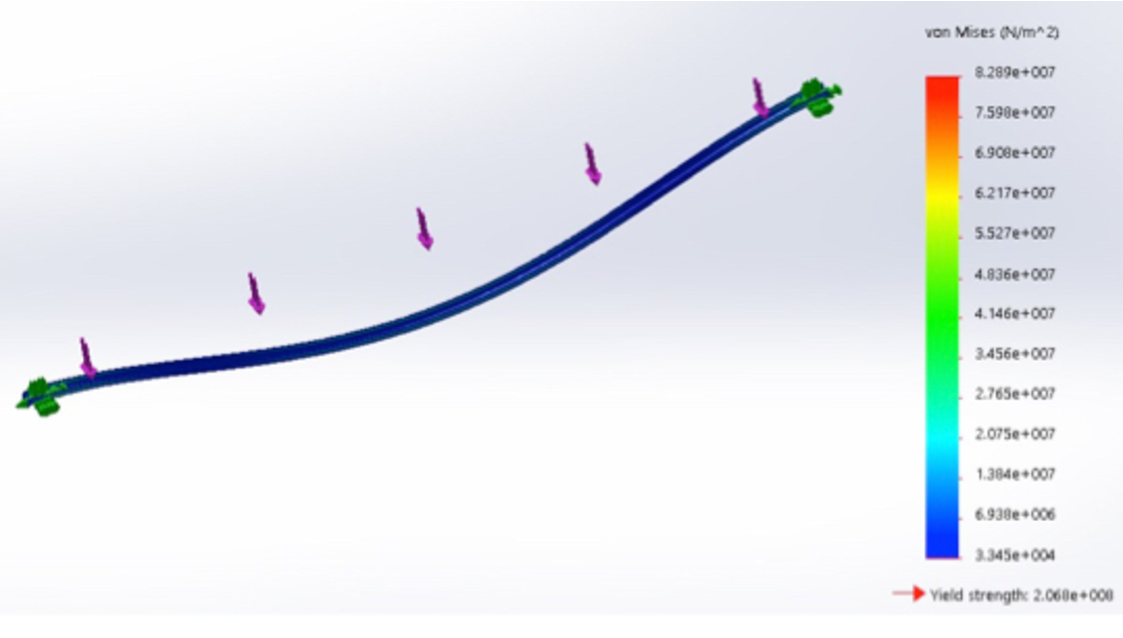
\includegraphics[width=0.25\columnwidth]{pds-rail-stress-apa-vert.pdf}
\end{dunefigure}


%%%%%%%%%%%%%%%%%%%%%%%%%%%%%%%%%%
\subsection{Photosensors and Photosensor Modules}
\label{sec:fdsp-pd-assy-psm}
%\metainfo{\color{blue} Content: Zutshi/Cancelo/Moreno?}

%The use of \dwords{sipm} in noble liquids is relatively young but rapidly growing field with experiments such as GERDA, MEG II, Darkside, nEXO etc. in various stages of preparation. 
The use of \dwords{sipm} in noble liquids is relatively new, but growing rapidly with experiments such as GERDA, MEG II, Darkside, and nEXO in various stages of preparation.
DUNE will learn a great deal %immensely 
from them, but in principle imposes even more stringent accessibility and longevity constraints. Risk mitigation through reliability engineering, process control, and vendor and collaboration testing will be a key feature of the DUNE \dword{sipm} production process.

{\textit{Reliability Engineering:}} The primary issue is the changes in material properties and thermal stresses induced in the packaging due to differential coefficients of thermal expansion (CTEs). This is especially critical for interfaces, in particular %with the relevant ones in this case being 
die-to-substrate, substrate-to-potting mold, potting mold-to-encapsulation and solder joints-to-everything else. Analysis of these interfaces and collaboration with vendors to match CTEs as much as possible at these interfaces will contribute substantially to the long-term reliability of the photosensors.

{\textit{Process Control:}} Small and seemingly innocuous %superficially innocuous seeming 
changes in the photosensor fabrication process can have a big impact on the robustness of these devices at extreme temperatures. This is one of the reasons why in space applications, for instance, same-day same-batch components are utilized. Given the photosensor quantities involved, this %criteria is not a practical option 
is not feasible for the DUNE \dword{pds}, but %does imply an 
it will be important to establish an MoU with the vendor regarding %in terms of 
strict process control once the pre-production batch has been qualified.

{\textit{Quality Assurance:}} This will be an essential component in the photosensor risk mitigation strategy consisting of restricting the number of production batches, clearly communicating desired device and packaging parameters to the vendor, and vendor testing to 
%warrant 
guarantee device operation down to liquid nitrogen temperatures. %This requirement implies that, b
Before shipment to the collaboration, the vendor %will 
must qualify a randomly selected sample of devices from each production batch. The qualification would entail thermally stressing the devices %and before/after 
with visual and electrical measurements made before and after. 

{\textit{Quality Control:}} The above strategies, while significantly lowering the risk, do not obviate the need for a strict testing regimen. Every sensor will be tested multiple times, at various stages of assembly, before installation in the \dword{spmod}.

\Dwords{sipm} are mounted in groups of six passively-ganged sensors to mounting boards, with eight mounting boards per supercell.  Passive ganging (sensors in parallel) is implemented with traces on the \dword{sipm} mounting board (\dword{pd} module), % and has been implemented 
as was done for \dword{pdsp}.  The \dwords{sipm} are mounted using a pick-and-place machine and standard surface-mount device soldering procedures. The outputs from these mounting boards are then routed to active ganging circuits in the center of the \dword{pd} module, where they are collected into a summing amplifier and reduced to a single output channel.

%\fixme{Is the following a Production and Assembly topic?}
%\fixme{Dave W--  I think this should stay here--  it is a design feature}
% rjw 12/4/18 ok

The ganged analog signals %are then brought out 
exit via long cables (approximately \SI{25}{m}) for digitization outside the cryostat.
\dword{pdsp} has provided essential operational experience with a passive ganging board and signal transport provided by Teflon Ethernet CAT6 cables.
R\&D is needed to optimize the connectors used to couple the cable to the board;  it is a priority to understand the mechanical stresses involved in the \dword{sipm}-PCB-connector system (with different CTEs) as it is cooled (or cycled) to cryogenic temperatures.


%%%%%%%%%%%%%%%%%%%%%%%%%%%%%%%%%%
\subsection{Electronics}
\label{sec:fdsp-pd-assy-pde}
%\metainfo{\color{blue}  Content: Moreno/Franchi/Djurcic}

The \dword{pds} consortium gained extensive experience in manufacturing processes %was gained 
during the development of the \dword{pdsp} \dwords{ssp}. % used on , 
A general description of the readout system of \dword{pdsp} can be seen in the Section~\ref{sec:fdsp-pd-pde}. Compatibility between elements designed by different institutions is guaranteed when standard procedures are followed, so the circuit design must be done in accordance with mutually agreed-upon specification documents.  A sufficient  number of units must be produced to allow %local testing and 
for testing both locally and  in the central facility; for example, in \dword{pdsp} five 12-channel  \dwords{ssp} were produced and delivered to CERN for integration testing. Twenty-four were fabricated for \dword{pdsp} operation. 

The readout electronics of the \dword{pds} will be designed and produced with similar tools and protocols as for  \dword{pdsp}. For example, %printed circuit board (
PCB layout is performed in accordance with IPC\footnote{IPC\texttrademark{}, Association Connecting Electronics Industries, \url{http://www.ipc.org/}.} specifications. Bare PCB manufacturing requirements are embedded within the Gerber file 
%\{Gerber needs TM?} - no it is a open file format
fabrication documents (e.g., layers, spacing, impedance, finish, testing, etc.). Components are assembled on circuit boards either by trained \dword{pd} consortium technical staff or by external assembly vendors, based on volume, and in accordance with per-design assembly specification documents. Testing occurs at %labs and universities within the 
collaboration institutions in accordance with a per-design test procedure that typically includes a mix of manual, semi-automated and automated procedures %testing 
in an engineering test bench followed by overall characterization in a system or subsystem test stand.
Other considerations and practices relevant to readout electronics production and assembly are itemized here:

\begin{itemize}

\item Components: Schematic capture is done using appropriate tools (such as OrCAD 16.6.\footnote{OrCAD\texttrademark{} schematic design tool for PCB design http://www.orcad.com} or similar toolset) available within a design facility. Design is hierarchical with common \dword{fe} page referenced multiple times ie for all input channels. 
%\fixme{clarify prev sentence}
The schematic contains the complete bill of materials (BOM) including all mechanical parts. An electronics schematics subversion
% \fixme{SVN? remember subversion has other meanings!}
repository or similar tool is typically used for version control and backup. Multiple internal design reviews are held before the schematic is released %to 
for layout. The BOM, stored directly within the schematic, is extracted to a spreadsheet when ordering parts. Every part specifies %is specified by 
both manufacturer and distributor information. Distributor information may be overridden by a technician at order time due to price or availability. Standard search engines such as Octopart\footnote{Octopart https://octopart.com/}, ECIA\footnote{ ECIA https://www.eciaauthorized.com} and PartMiner\footnote{PartMiner https://www.part-miner.com/} are used to check price or availability across all standard distributors. A parts-availability check %review 
is performed prior to handoff from schematic to layout since % as required 
obsolete or long lead-time parts %were 
may have been removed from the design and replaced. BOM information includes dielectric, tolerance, temperature coefficient, voltage rating, and size (footprint) to ensure that all parts are fully described.

\item Boards: Standard tools (such as the Allegro\footnote{Cadence Allegro\textregistered PCB design solution https://www.cadence.com} toolset) are available for the PCB layout. Conventional PCBs are %realized as multilayer boards with controlled impedance 
controlled-impedance multilayer boards with many sets of delay-matched nets where necessary. %In usual practice the complete impedance and delay characteristics are calculated within layout tool and crosschecked by PCB vendor prior to manufacture. In usual practice, a competitive bid between multiple previously qualified vendors is used, with a full electrical and impedance testing required. Multiple internal design reviews are held prior to release of the design.
In usual practice, multiple previously qualified vendors bid competitively. The consortium electronics group provides the complete impedance and delay characteristics  within the layout tool, and the selected vendor cross-checks these values prior to manufacture and performs full electrical and impedance testing.  Multiple internal design reviews are held prior to release of the design.

\item Cable plant: The cabling designed will take into consideration the \dword{apa} space and will be done in close collaboration with the TPC \dword{ce} consortium to avoid crosstalk effects. %A final decision on cable procurement will be taken based on 
Before making a final decision on cable procurement, we are investigating the possibility of cable manufacturing in a \dword{pds} consortium institution versus the cost of a commercial solution.  

\item Manufacturer list: In addition to the general laboratory procedures for \dword{qa}, the general practice will be to use only PCB manufacturers and external assembly vendors whose workmanship and facilities have been personally inspected by experienced production team members. All external assemblers are required to quote in accordance with an assembly specifications document describing the IPC class and specific solder chemistry requirements of the design. The BOM document will show selected and alternate suppliers where available for every component of the \dword{fe} boards.

\item \dword{fe} electronics firmware: This will be specified and updated iteratively in collaboration with other systems. The electronics working group will be responsible for responding to requests for additional firmware development, including for example, modifications to timing interface, modifications to trigger interface, and implemented sensitivity to in-spill versus not-in-spill conditions. Documents describing firmware architecture for each major change will be written and distributed to \dword{pd} and \dword{daq} working groups before implementation. A \dword{fe}  electronics users manual containing all details of new firmware will be distributed with production units when manufactured.

\item Mechanical assembly: With the mechanical assembly of electronics readout boards it is common practice to use a \threed model generated by the layout software.  %AutoCAD\footnote{AutoDESK AutoCAD\textregistered computer aided design software application https://www.autodesk.com/} or similar software with Allegro (as PCB layout tool). 
All relevant dimensions of the PCB including connector and indicator placement is extracted as a base DXF file from which an overall exploded mechanical diagram of chassis and other mechanical parts is made.  Mechanical items such as shield plates will also be provided. It is assumed that external vendors will make the \dword{fe} chassis %will made by external vendors 
(one for the chassis, one for front and back panels) from drawings provided by the consortium.

\end{itemize}

\subsection{Calibration and Monitoring}
\label{sec:fdsp-pd-assy-CandM}
%\metainfo{\color{blue}  Content: Djurcic}

The consortium gained extensive experience in manufacturing, testing and assembly processes %was gained 
during the development of the calibration and monitoring system for \dword{pdsp}.
A general description of the proposed calibration and monitoring system can be seen in  Section~\ref{sec:fdsp-pd-CandM}. 

%The design and production of the calibration modules with electronics circuitry, with \dword{fpga} implementation for light-source controls and with optical timing/trigger and \dword{daq} communication protocols, with implementation of UV light sources, follows closely the process described in Section~\ref{sec:fdsp-pd-assy-pde}.
The design and production of the calibration modules including electronics circuitry,  \dword{fpga} implementation for light-source controls, optical timing/trigger and \dword{daq} communication protocols, and UV light sources, closely follows the process described in Section~\ref{sec:fdsp-pd-assy-pde}.

Design and selection of cold diffuser components and selection of cold and warm quartz fiber components follows requirements derived from interface considerations with \dword{hv},  \dword{cpa} and cryostat systems, %HV/CPA and Cryostat systems, 
and was tested in \dword{pdsp}.
Installation, \dword{qa} and \dword{qc} of optical fibers is performed during the \dword{cpa} installation process, with diffusers and \dword{cpa} fibers pre-installed with \dword{cpa}s.

Installation of fibers that connect \dword{cpa}s %'s fiber connections 
to the optical feedthrough penetrations at the cryostat will be defined with the \dword{dss} and cryostat teams, based on installation experience in \dword{pdsp}. 